\documentclass[11pt,mathserif]{beamer}
\usetheme{Madrid}
%\usepackage{beamerthemesplit}
%\usepackage{beamercolorthemesidebartab}
\usepackage[utf8]{inputenc}
\usepackage[T1]{fontenc}
\usepackage{textcomp}
\usepackage{ngerman}
\usepackage{graphicx}
\usepackage{multimedia}
\usepackage{lmodern}
\usepackage{alltt}
\usepackage{epsfig,psfrag}
%\usetheme[usetitleprogressbar,nooffset]{m}
%\usetheme{Copenhagen}
%\usetheme{CambridgeUS}
%\setbeamercovered{transparent}
%\PrerenderUnicode{}
%\logo{\includegraphics[width=2cm]{logo_modern.pdf}}
%\setbeamertemplate{navigation symbols}{}
%\setbeamertemplate{footline}{}

\usepackage{natbib}
\usepackage{amsmath}
\usepackage{amsthm}
\usepackage{amssymb}
\usepackage{relsize}

\usepackage{xfrac}

% For algorithms
\usepackage{algorithm}
\usepackage{algorithmic}


\DeclareMathOperator*{\argmax}{argmax}

\graphicspath{{../arxiv/figures/}}

%\renewcommand{\vec}[1]{{\mathbf{#1}}}
\renewcommand{\vec}[1]{{\boldsymbol{ #1}}}
\newcommand{\Bernoulli}{\mathcal{B}}
\newcommand{\DD}{{\cal D}}
\newcommand{\LL}{{\cal L}}

\newcommand{\E}[2]{\mathop{\mathlarger{\mathbb{E}} }_{#1}\left[#2\right]}
\newcommand{\prob}[2]{p\left(#1 \, | \, #2\right)}
\newcommand{\qrob}[2]{q\left(#1 \, | \, #2\right)}

\newcommand{\kk}{{(k)}}
\newcommand{\mm}{{(l)}}
\newcommand{\ps}{p^*}
\newcommand{\pts}{\tilde{p}^*}
\newcommand{\ph}{\hat{p}}
\newcommand{\phs}{\hat{p}^*}
\newcommand{\x}{\vec{x}}
\newcommand{\y}{\vec{y}}
\newcommand{\z}{\vec{z}}
\newcommand{\h}{\vec{h}}
\newcommand{\norm}[1]{||{#1}||_2}
\newcommand{\Li}[1]{\mathcal{L}ip_{#1}}

\newcommand{\xVec}{\vec{x}}
\newcommand{\hVec}{\vec{h}}
\newcommand{\yVec}{\vec{y}}
\newcommand{\aVec}{\vec{a}}
\newcommand{\bVec}{\vec{b}}

\DeclareMathOperator*{\argmin}{arg\,min}


\title[]{Autoencoder}

\author{
  Asja Fischer \\
  Ruhr-Universi\"at Bochum\\
  asja.fischer@rub.de 
 % \includegraphics[width=0.4\linewidth]{people.png}
}
\date{04.07.2018}

\begin{document}

%\titlegraphic{\includegraphics[width=2cm]{logo_modern.pdf}}
\frame{\titlepage}

% \begin{frame}[fragile]
% \frametitle{Unsupervised Deep Learning}
% {\bf What can we learn from the success of deep supervised learning?}
% \begin{itemize}
%  \item Multiple layers of abstraction
%  \item Distributed representations
%  \item Flexible models with large capacity
% \end{itemize}
% \begin{center}
%   \includegraphics[width=0.5\linewidth]{layers01.pdf}
% \end{center}
% \end{frame}
%
% \begin{frame}[fragile]
% \frametitle{Unsupervised Deep Learning}
% {\bf What can we learn from the success of deep supervised learning?}
% \begin{itemize}
%  \item Multiple layers of abstraction
%  \item Distributed representations
%  \item Flexible models with large capacity
% \end{itemize}
% \begin{center}
%   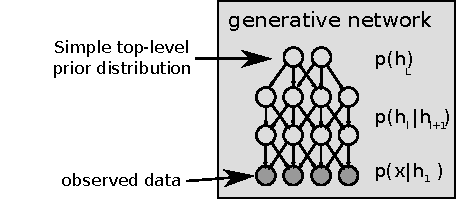
\includegraphics[width=0.5\linewidth]{layers02.pdf}
% \end{center}
% \end{frame}
%
%
% \begin{frame}[fragile]
% \frametitle{Unsupervised Deep Learning}
% {\bf What can we learn from the success of deep supervised learning?}
% \begin{itemize}
%  \item Multiple layers of abstraction
%  \item Distributed representations
%  \item Flexible models with large capacity
% \end{itemize}
% \begin{center}
%   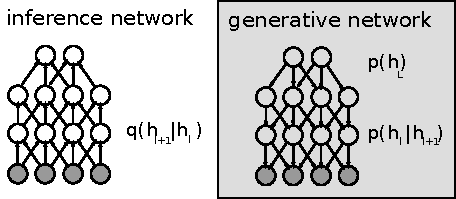
\includegraphics[width=0.5\linewidth]{layers.pdf}
% \end{center}
% \end{frame}

%%%%%%%%%%%%%%%%%%%%%%%%%%%%%%%%%%%%%%%%%%%%%%%%%%%%%%%%%%%%%%%%%%%%%%%%%%%%%
%\section{Supervised Deep Learning}

%\begin{frame}[fragile]
%\frametitle{Supervised Deep Learning}
%%\begin{center}
%
%Given labeled data $(\vec x_1, \vec y_1),(\vec x_2, \vec y_2),\dots (\vec x_S, \vec y_S)$ train a neural network with multiple layers to perform a regression or classification task. 
%
%\vspace{0.4cm}
% \hspace{0.1cm} 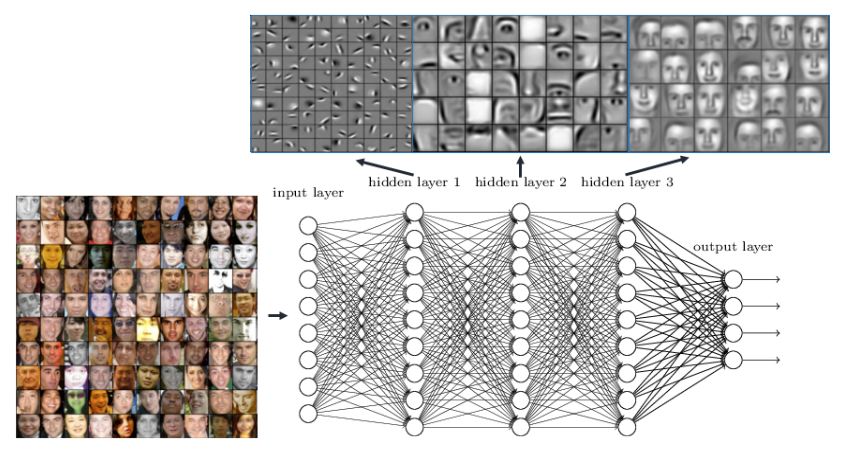
\includegraphics[width=0.9\framewidth]{SupDeepNet}
%
%\footnotesize{[Lee, Grosse, Ranganath and Ng, ICML, 2009]}

%deep learning is: Learning multiple levels of 
% to help a learner %accomplish a task of interest, with higher levels capturing more abstract %concepts through a deeper composition of computations.



 
%\end{center}
%\end{frame}


\frame{
\frametitle{Unsupervised Learning}

\begin{itemize}
\item 
%Training data: training data consists of unlabeled input points. TODO: 
Training data: A set of unlabeled i.i.d.~examples $x_1, x_2,\dots, x_n \sim p_{\text{data}}$. 
%sampled from unknown distribution. 
\item  Task: find and describe intrinsic structure in the data.
\end{itemize}

\vspace{0.5cm}
\hspace{2cm} clustering \hspace{2cm} density fitting  
\vspace{-1cm}
\begin{figure}
\centering
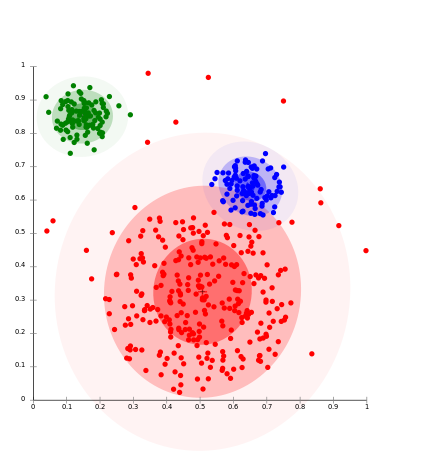
\includegraphics[width=5cm]{clustering.png}
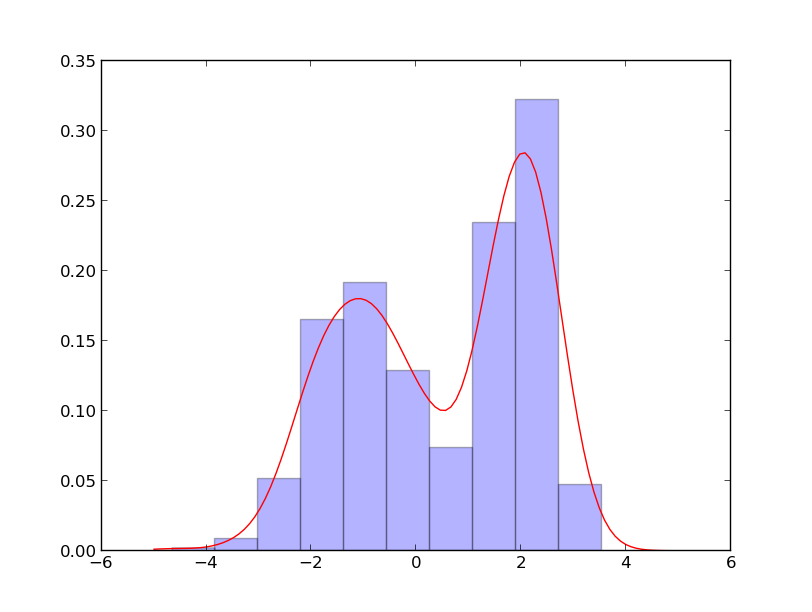
\includegraphics[width=6cm]{kerneldist.png}
\end{figure}
}

\begin{frame}[fragile]
\frametitle{Unsupervised Deep Learning}
Given i.i.d. (unlabeled) data $\vec x_1, \vec x_2,\dots, \vec x_S \sim  p_{\text{data}}$  train 

 \begin{itemize}
 
 \item  a model for \textbf{representation learning} (feature extraction, dimensionality reduction, manifold learning, ...).

 \pause
 
  \item a \textbf{generative model}, i.e. a probabilistic model of the  data generating distribution  $p_{\text{data}}$ 
  % (predictions, missing feature estimation, reconstruction, denoising, sampling, outlier detection, ...).
  (data generation, outlier detection, missing feature extraction, reconstruction, denoising or planing in reinforcement learning, ...). 
  
  %full probabilistic model of all variables
  
 \end{itemize}


\end{frame} 

\section{Representation Learning}

\subsection{Autoencoders}

\frame{\frametitle{Outline}\tableofcontents}

\begin{frame}
  \frametitle{Autoencoder (AE)}
  
TODO: Image!   
  
  \begin{itemize}
  \item AEs are a special kind of feed forward neural networks.
  \item  Task: reconstruction of  the input.     
  \item They consist of two parts:
  \begin{itemize}
            \item encoder function $\vec{h} = f(\vec{x})$
            \item decoder that produces the reconstruction $\hat{\vec{x}} = g(\vec{h})$
  \end{itemize}
    \item Loss function: $L\left(\vec{x}, g(f(\vec{x}))\right)$
    \item Goal: Learn good representations $\vec h$.
  \end{itemize}
  
  \end{frame}
  
 \begin{frame}
  \frametitle{Autoencoder (AE)}
  
  \begin{itemize}
  \item \textbf{Undercomplete} AE $:$ code dimension $<$ input dimension.
  \item  Example: For an undercomplete AE with 
  \begin{itemize}
  \item  linear decoder $g(\vec h)= \vec W \vec h$
  \item  mean squared error loss $L=||\vec x-g(f(\vec x))||^2_2$
  \item  input normalized to have zero mean
  \end{itemize}
  optimal encoder corresponds to Principal Component Analysis (PCA).
  \item AE with non-linear decoder/encoder can be seen as non-linear generalization of PCA.
  \item Problem: If AE is \textbf{overcomplete} (code dimension $>$ input dimension) or encoder and decoder are too powerful AE can learn to simply copy the input.
    
  \end{itemize}
  
 \end{frame}
  
  \begin{frame}
  \frametitle{Regularized Autoencoder}
  %\begin{overlayarea}  
    \begin{itemize}
      
       \item Regularized AEs modify the original loss function to:
       \begin{itemize}
       \item prevent from trivially copying the inputs 
       \item encourage additional properties
       \end{itemize}
       
     
       %    \pause
       %\item The model is encouraged to have additional properties
       %    \pause
        \item Examples:
            \begin{itemize}
                \item \textbf{Sparse AE:} sparsity of the representation
               %     \pause
                \item \textbf{Denoising AE}: robustness to noise %and outliers
             %       \pause
                \item \textbf{Contractive AE}: small derivatives of the representation w.r.t. input
                 %   \pause
            \end{itemize}
   
    \end{itemize} 
    %$\Rightarrow$ 
   % A regularized autoencoder can be overcomplete and nonlinear but still learn something useful about the data distribution!  
  
  
\end{frame}

  
 
\begin{frame}
  \frametitle{Denoising Autoencoder}
 
    \begin{itemize}
       \item Idea: representation should be robust to introduction of noise.
       \item Produce corrupted version $\tilde{\vec x} $ of  input $\vec x$ by
     \begin{itemize}  
        \item random assignment of subset of inputs to 0 
      \item adding Gaussian noise 
       \end{itemize}
        %\item 
        \item Modified reconstruction loss: $L(\pmb{x}, \alert{g(f(\tilde{\pmb{x}})})$ %instead of $L(\pmb{x}, g(f(\pmb{x}))$   
            %\begin{itemize}
            %\item $\tilde{\pmb{x}}$ is a copy of $\pmb{x}$ corrupted with some form of noise\\
           % \end{itemize}
          %  $\Rightarrow$ denoising autoencoders must learn to undo this corruption \\
         %   $\Rightarrow$ $f$ and $g$ implicitly learn the structure of $p_{data}(\pmb{x})$
    \end{itemize}

TODO: Image!    
    
\end{frame}


%\begin{frame}[t]{Denoising Autoencoder -Training Procedure}
  %  \begin{columns}
  %      \column{0.3\linewidth}
    %    \begin{figure}[h]
    %        \centering
  %      \includegraphics[scale=.23]{resources/figure14-3.png}
   %         \caption{The computational graph of the cost function for a denoising autoencoder.}
   %     \end{figure}
        % \column{0.3\linewidth}
        % \includegraphics[scale=.23]{resources/figure14-3.png}
     %   \column{0.7\linewidth}
%        \begin{itemize}
%         %   \pause
%            \item Introduce a corruption process $C( \pmb{\tilde{x}} \mid \pmb{x})$ 
%        %    \pause
%            \item The autoencoder then learns a \textit{reconstruction distribution} $p_{reconstruct}(\pmb{x}\mid\tilde{\pmb{x}} )$ as follows:\\
%        %    \pause
%                \begin{enumerate}
%                    \item Sample a training example $\pmb{x}$ from the training data
%        %    \pause
%                    \item Sample a corrupted version $\pmb{\tilde{x}}$ from $C( \pmb{\tilde{x}} \mid \pmb{x})$
%       %   \pause
%                    \item Use $(\pmb{x},\pmb{\tilde{x}})$ as a training example for estimating the autoencoder reconstruction distribution $p_{reconstruct}(\pmb{x}\mid\pmb{\tilde{x}} ) = p_{decoder}(\pmb{x}\mid\pmb{h})$ 
%
%                \end{enumerate}
%        \end{itemize}
%%    \end{columns} 
%\end{frame}

%\begin{frame}[t]{Denoising Autoencoder - Training Procedure}
%    \begin{figure}[h]
%        \centering
%     \includegraphics[width=0.8\linewidth]{figure14-4.jpg}
%        \caption{A denoising autoencoder is trained to map a corrupted data point $\tilde{\pmb{x}}$ back to
 %       the original data point $\pmb{x}$
 %       TODO: Referenz statt Caption?} 
%    \end{figure}
%\end{frame}



\begin{frame}[t]{Contractive Autoencoder}
   \begin{itemize}
       %\item Remember: contractive autoencoders are regularized autoencoders
   %     \pause
       \item Idea: extract features that only reflect variations found in the training set.
   %     \pause
       \item Add explicit regularization term 
       %on the code $\pmb{h}$
        to the reconstruction loss:\\
           \begin{center}
       $L(\pmb{x}, g(f(\pmb{x})) + \alert{\lambda \Vert \frac{\partial f(\pmb{x})}{\partial \pmb{x}} \Vert^2_F}$ 
   \end{center}
   
%        \pause
  $\Rightarrow$  Derivatives of the encoder function w.r.t.~the input are encouraged to be small.
%        \pause
%    $\Rightarrow$ Only a small number of input directions will have significant derivatives\\ 
%        \pause
 %  $\Rightarrow$ The encoder function is encouraged to resist infinitesimal perturbations of the input
   \end{itemize} 
\end{frame}

\begin{frame}
\frametitle{Which Autoencoder?}

\begin{itemize}
\item Both the denoising and contractive autoencoder perform well
\item Advantage of denoising autoencoder : simpler to implement
\begin{itemize}
\item  requires adding one or two lines of code to regular 
\item autoencoder no need to compute Jacobian of hidden layer
\end{itemize}
\item Advantage of contractive autoencoder: gradient is deterministic
\begin{itemize}
\item can use second order optimizers (conjugate gradient, LBFGS, etc.)
\item might be more stable than denoising autoencoder, which uses a sampled gradient
\end{itemize}
\end{itemize}

\end{frame}

%\begin{frame}[t]{DAE's vs. CAE's}
%    \begin{table}[h!]
%        \centering
%        \label{tab:}
%        \begin{tabular}{p{5cm}|p{5cm}}
%            \textbf{DAE} & \textbf{CAE}\\
%            \hline
%%            \pause
%            the \textit{decoder} function is trained to resist infinitesimal perturbations of the input & \pause the \textit{encoder} function is trained to resist infinitesimal pertubations of the input
%        \end{tabular}
%    \end{table}
%\end{frame}

\



\end{document}
